\documentclass[]{article}

\usepackage{amsfonts}
\usepackage{amsmath}
\usepackage{graphicx}
\usepackage{amsthm}
\usepackage{svg}
\usepackage{enumitem}
\usepackage{color}
\usepackage{float}

\graphicspath{{images/}}
\setsvg{svgpath={./images/}}

\newtheorem{thm}{Theorem}[subsection]
\newtheorem{Def}{Definition}[subsection]
\newtheorem*{thm*}{Theorem}
\newtheorem*{def*}{Definition}

\newcommand{\compav}[1]{\textbf{\textcolor{blue}{#1}}}
\newcommand{\compat}[1]{\textbf{\textcolor{red}{#1}}}
\newcommand{\shiftleft}[2]{\makebox[0pt][r]{\makebox[#1][l]{#2}}}
\newcommand{\tilda}{\big{\char"7E}}


%opening
\title{Geodesic Flow on the Necker Cube Surface}
\date{}
\author{Pavel Javornik}

\begin{document}


\maketitle



\begin{center}

\includesvg[width=4.8in]{cubecoverphoto}\\
\end{center}

\begin{abstract}
This paper classifies the periodic and drift-periodic trajectories on the Necker cube surface, a periodic surface built out of squares popular in optical illusions.
\end{abstract}



\newpage
\section{Introduction}

The purpose of the following paper is to study the geodesic flow on the periodic surface depicted above, which is formed from an infinite collection of unit squares. We call this surface the Necker cube surface after Louis Albert Necker's ``Necker Cube$_{1}$,'' which became a popular optical illusion. M.C. Escher's adaptation of the cube in Metamorphosis I$_{2}$ briefly features the Necker cube surface (See Figure $\ref{fig:Escher}$).The term Necker Cube is used interchangeably to refer to Escher's surface adaptation and Necker's optical illusion. For the purposes of the following paper, we will be using either Necker Cube or $\mathbf{S}$ to refer to the periodic cube tiling that appears in Escher's work.


\begin{figure}[H]
\begin{center}
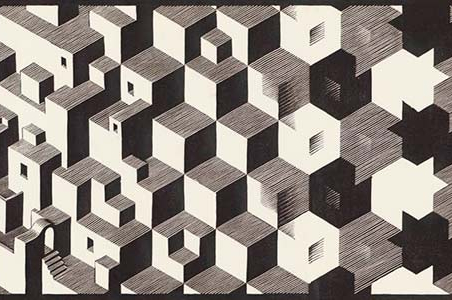
\includegraphics[scale=0.5]{escher.jpg}
\caption{The Necker cube as it appears briefly in Metamorphosis I}
\label{fig:Escher}
\end{center}
\end{figure}

The initial (rational) trajectories of any given flow fall into only one of two categories.
\compat{The definitions below seem redundant. Perhaps you want ${\mathcal O}$ and ${\mathcal E}$}

\begin{def*}
Let $v$ be a vector of the form $(x,y)\in\mathbb{Z}^{2}$. We call $v$ an \textbf{odd-odd} vector if x and y are relatively prime and both odd. We denote the \textbf{set of all odd-odd vectors} by $\mathcal{O}$. We say that $v$ is an  \textbf{even-odd} vector if x and y are relatively prime, and x is even if and only if y is odd. We denote the \textbf{set of all even-odd vectors} by $\mathcal{E}$.
\end{def*}

We consider every (rational) initial trajectory on the surface to fall into one of the two categories, otherwise it is a positive scalar multiple of some direction. Given some initial point $x_{0}$ on the surface embedded in real space and some vector direction in real space, $\bar{v}$, our initial trajectory,$v$, is taken as an isomorphism from the planar subspace of $\mathbb{R}^{3}$ that contains $\bar{v}$. The three possible cases are the auxiliary planes, $x=0, y=0, z=0$, whose projections onto $\mathbb{R}^{2}$ are given by $(0,y,z)\mapsto(-z,y)$, $(x,0,z)\mapsto(x,-z)$, and $(x,y,0)\mapsto(x,y)$ respectively and relative to the standard bases of $\mathbb{R}^{3}$. We take $-z$ to be positive, and consider vectors that lie outside of these subspaces as degenerate cases. From there we prove the following:

\begin{thm*}{Given an initial trajectory, $\theta\in\mathbb{R}^{2}$, and geodesic path, $\gamma$, on $\mathbf{S}$ with initial trajectory $\theta$, the following is true:} \compat{There is no flow in a fixed direction because when trajectories move to new squares they may be traveling different directions.}
\compav{Can I use gamma as a path on S?}
\begin{enumerate}[label=(\roman*)]
\item If $\theta$ belongs to $\mathcal{O}$, then $\gamma$ is closed on $\mathbf{S}$ and homeomorphic to $\mathbb{R}/\mathbb{Z}$.
\item If $\theta$ belongs to $\mathcal{E}$, then $\gamma$ is drift-periodic on $\mathbf{S}$.

\end{enumerate}
\end{thm*}

\compav{Archiving for later:\\If $\theta$ is of the form (x,y) such that x or y are irrational, then $\phi^{\theta}_{t}$ is uniquely ergodic on $\mathbf{S}$. \compat{We should move the discussion of ergodicity outside the theorem.}	}

\compav{Stopped here. Continued in Section 2.}

The Necker Cube is a member of the family of infinite Euclidean cone surfaces built out of rectangles with vertices of cone angle $3\pi$ and $\frac{3\pi}{2}$. We wish to study the surface in the case where we glue only squares with edges of length 1. Specifically, we want to study geodesic flows on this surface and to prove that properties of the initial trajectory angle determine whether or not the geodesic will close or drift periodically. 

The determining factor is simply whether or not the trajectory angle vector direction $(a,b)$, relative to the bottom and left edges of any square face, has integer values $a$,$b$ (where $a$ and $b$ are relatively prime) are of the same parity (odd-odd slope) or different parities (even-odd slope). We choose to neglect cases where paths are incident with vertices, and proceed to treat them as singularities. With these conditions in place we found that any geodesic with an initial odd-odd trajectory closes on the surface, while the even-odd cases drift periodically, tending to infinity. We aim to prove the following:



\subsection{Discussion of Proof}
\subsection{Related work}


To better understand this surface, we will adapt methods used in the study of Veech surfaces to suit our needs. These methods have become incredibly valuable to anyone studying rational billiard flows on a variety of compact or (in the case of infinite surfaces) non-compact surfaces. Geodesic flows in these problems are characterized as point masses moving along frictionless surfaces that experience perfectly elastic collisions with the boundaries of the surface. The straight line path is then deformed by a reflection over the boundary in the opposite direction. Translation surfaces constructed in the following manner therefore take on symmetric properties in accordance to these transformations and the types of boundaries the point mass might encounter. That is to say that orienting these flows requires that the translation surface itself be reflected to realign the flow. These translation surfaces are often described as being "unfolded" by some billiard flow, or strung along a laundry line of polygons congruent to the base. In the later sections we will describe how our surface's canonical form deforms geodesic flows by rotation and how we can use these rotations and edge-crossings to determine whether or not a geodesic will close.

What inspired this paper was the work done by Hubert et al. [Hu] on the Ehrenfest-Wind Tree model. Any readers who are familiar with their paper or the Tree model will most likely notice the similarities between the quotient spaces of the two surfaces and the properties that determine whether or not geodesic paths close. While similar, these surfaces are not entirely identical. The effect that a boundary collision has on a geodesic alters the dynamical properties of the surface. Or perhaps they better demonstrate properties of the surface itself. Another fundamental difference between the two is that the Necker Cube is a surface with cone angles surrounding an infinite number of singularities on the surface. The problem has to take into careful consideration what it means for a path to cross a saddle connection between these singularities of the translation surface.



\subsection{Procedure}
The Necker Cube surface has an interesting construction process that lets us take each face of the cube and arrange them in any way we choose so long as we do not change how the edges are identified, or glued together. It is preferable to study the flows on this surface as though every cube has been flattened onto the plane. This means that we can consider the cube step to be tiled by infinitely many of L-shaped surfaces whose edges are identified by rotation.

Doing so greatly reduces the number of possible directions that a flow might travel. Since every edge of this L-shaped surface is identified to another either by translation or a 90 degree rotation, any straight line path on this flattened version of the Necker Cube can experience only one of four possible directions at any given time, whereas the Necker Cube would've had considerably more.

Moreover, every face of this L-shaped surface is given by rotating its associated face on the Necker Cube about the x or y axis, affine translations, or a combination of the two. By cutting and gluing every half-cube of the Necker Cube in a consistent fashion, we can preserve the areas of the faces and distances between any two points on the surface with the flattening procedure. We describe this procedure as piecewise maps that are comprised of compositions of Euclidean matrices and translations of points relative to the L-shape onto a subset of $\mathbb{R}^{2}$ with square shaped holes cut out. Since rotations and translations of points preserves distance between them, the path lengths and  associated properties of geodesic flows remain invariant.

The image of this map is a flattened version of the Necker Cube. (See FIG [MATLAB MODEL]). From that surface we construct a new one made out of four copies of original, each rotated by some factor of 90 degrees so as to realign the geodesic flows and assure that they can only travel in one possible direction. This four-fold surface is then a cover of the original surface. We consider every possible direction to be a "phase" of the flow, and index the planes accordingly. Any edges in the holes of the surface are identified with an edge on an adjacent phase plane (By rotation of $\pm \frac{\pi}{4}$). Any point on this surface has a coordinate in $\mathbb{R}\times\mathbb{R}\times\mathbb{Z}_{4} $

Similarly, we take the quotient space of the flattened Necker Cube centered around each square shaped hole and realign its flows by rotation. The resulting surface is a compact branch cover of the quotient space. Singularities on the translation surface have a total angle that is some multiple of $2\pi$. We consider the translation surface to be a base surface of the four-fold cover, and study its properties to prove our main theorem. In particular, we wish to determine what effect a member of the translation surface's Veech group has on both the surface and geodesic flow in hopes that it would shine some light on odd-odd even-odd phenomenon.



 $SL_{2}(\mathbb{R})$

\section{Constructing the Surface \& Isometric Variant}
\compav{Started up here again 6/21/17}

This section will detail how the Necker cube (See Figure \ref{fig:cubexyz}) is constructed out of an infinite set of unit squares, and explain the process by which we flatten the structure in such a way that preserves distances, and makes it simpler for us to describe the behavior of the geodesic flows that come into contact with these edges.

\begin{figure}[H]
\begin{center}
\includesvg[width=3in]{cubesxyz}
\caption{The Necker cube embedded in space.}
\label{fig:cubexyz}
\end{center}
\end{figure}

\subsection{The Necker Cube Surface}

To build the surface out of infinitely many unit squares, we take the union of the instances of three squares, each lying on planes orthogonal to the other two and sharing an edge with exactly one other square. The three squares have only one vertex in common.

First we divide the planes $x,y,z=k$ for some integer $k$ in such a way that they are composed entirely out of unit squares. We want to index each of these squares by integer triples and some label A,B, or C. i.e. squares on planes of the form $z=k$ will have an A label, $x=k$ a B label, and $y=k$ a C label. Let $m,n,p\in\mathbb{Z}$. Then each square based at $(m,n,p)$ is defined as follows:

\vspace{0.2in}
\begin{tabular}{p{10cm}c}
\begin{align*}
\mathbf{A}_{m,n,p} = [m, m+1]\times[n,n+1]\times\{p\} 
\\\mathbf{B}_{m,n,p} = \{m+1\}\times[n,n+1]\times[p-1,p]
\\\mathbf{C}_{m,n,p} [m,m+1]\times\{n+1\}\times[p-1,p]
\end{align*}
&
\shiftleft{0.8in}{\raisebox{-1in}{
\includegraphics[scale=1]{label.png}}}
\end{tabular}
\vspace{0.2in}
\compat{I would define $A_{m,n,p}$, etc.}\\
\noindent For the sake of convenience, B and C are shifted in order to associate each integer triple that satisfies the linear condition $m+n+p=0$ with an instance of the cube that $\mathbf{S}$ is composed of. Furthermore, we can separate $\mathbf{S}$ into the sets:

\begin{align*}
\mathbf{A}=\bigcup\big{\{}\mathbf{A}_{m,n,p}: m+n+p=0\big{\}}
\\\mathbf{B}=\bigcup\big{\{}\mathbf{B}_{m,n,p}: m+n+p=0\big{\}}
\\\mathbf{C}=\bigcup\big{\{}\mathbf{C}_{m,n,p}: m+n+p=0\big{\}}
\end{align*}

\noindent We can now give a formal definition of the Necker Cube.

\begin{Def}{The Necker Cube.} 
\\ The \textbf{Necker Cube}, denoted by $\mathbf{S}$, is the surface made up of unions of unit squares of the form $\mathbf{S} = \mathbf{A}\cup\mathbf{B}\cup\mathbf{C}$.\end{Def}

\noindent $\mathbf{S}$ is the surface portrayed in Figure \ref{fig:cubexyz}. 

\subsection{The Flattened Form}
We will show that $\mathbf S$ is isometric to a a topological quotient of a particular subset of the plane. We call this surface $\mathbf{U}$, and the subset of the plane $\mathbf P$ (See Figure $\ref{fig:uprimeu}$).

\begin{Def}{$\mathbf{P}$}\\
$\mathbf P$ is the region of the plane with unit squares removed:
$$\mathbf{P} = \mathbb{R}^{2}\text{ }\backslash\bigcup_{m,n \in {\mathbb Z}} \big{\{}(u,v):u\in(2m-\frac{1}{2},2m+\frac{1}{2}),\text{ } v\in(2n-\frac{1}{2},2n+\frac{1}{2})\big{\}}$$
\end{Def}

\begin{figure}[H]
\begin{center}
\includesvg[width=1.5in]{uprime}
\end{center}
\caption{$\mathbf P$, the subset of the plane with unit squares removed at every even integer pair.} \compat{Perhaps just use one.}
\label{fig:uprimeu}
\end{figure}

\noindent On $\mathbf P$ we define a relation that identifies the sides of the boundaries of each hole in the plane with another by rotating an edge around the bottom left or top right corners by $\pm\frac{\pi}{2}$. The result is an edge identification as seen here (centered at each even coordinate pair):

\begin{figure}[H]\centering
\includesvg[width=2in.]{quotient}
\end{figure}
\noindent We call this relation $\mathbf{R}$. What $\mathbf{R}$ essentially does is translates every hole to the origin and identifies the edges by reflecting over the line $y=x$. If these points coincide, then they are indeed the same point on the boundary. Otherwise, every point that is not on the boundary belongs to its own class. We can safely assume this wont identify edges improperly, since we translate every boundary so as to situate the unit holes over the origin. For example, if we took two edges that do not belong to the same hole then by that same translation and reflection the two edges couldn't possible coincide. 

\begin{Def}
content...
\end{Def}

\begin{Def}{$\mathbf U$}\\
$\mathbf U$ is equal to the quotient space $\mathbf{P}/\mathbf{R}\times\{0\}$
\end{Def}

\compav{Stopped here. 6/21/17}

\compat{I would use as an introductory paragraph: ``We will show that $\mathbf S$ is isometric to a topological quotient of a subset of the plane.''}

Before describing the transformation that takes $\mathbf{S}$ to its flattened form, it would be best to define the relations on a subset of the plane that preserves the identification of edges. We will call this surface $\mathbf{U}'$. However, the flattening of the surface takes $\mathbf{S}$ to a translation of $\mathbf{U}'$, we call $\mathbf{U}$ (See $\ref{fig:uprimeu}$). We will denote the metric preserving map from $\mathbf{S}$ to $\mathbf{U}$, by $\Psi$. Defining these edge identifying relations over $\mathbf{U}'$ is more convenient for us than defining them over $\mathbf{U}$, but defining $\Psi$ is more convenient when the map is taken to $\mathbf{U}$ due to the nature of the construction of $\mathbf{S}$. \compat{I found this paragraph awkward. I would just go ahead and define the region in the plane.}



Now we will describe exactly how to construct $\mathbf{U}'$. Take the subset of the real plane, 
$$,$$ 
\compat{I would write $(m-\frac{1}{2},m+\frac{1}{2}) \times (n-\frac{1}{2},n+\frac{1}{2})$.}
with open unit squares cut out at every even integer pair and let $\mathbf{U}'$ represent the flattened structure with the proper edge identifications with the first "hole" centered at the origin. We will describe this surface as a cross product of the auxiliary plane, $z=0$ and the image of the natural map from $\mathbf{P}$ to its quotient space with the following relation on $\mathbf{P}$:

\begin{gather*}
\text{Let } x_{0}=(u_{0},v_{0}),x_{1}=(u_{1},v_{1}) \in \mathbf{P}. \text{Let } \mathbf{R} \text { be a relation given, } x_{0}\mathbf{R}x_{1} \\ \text{ iff } x_{0}=x_{1}
 \text{ or if }x_{0},x_{1} \in {\partial} \left( \left[2m-\frac{1}{2},2m+\frac{1}{2}\right] \times \left[2n-\frac{1}{2},2n+\frac{1}{2}\right] \right)\\
  \left[\begin{array}{c}
u_{1} -2m
\\v_{1}-2n
\end{array}\right] = \left[\begin{matrix}
0 && 1\\
1 && 0
\end{matrix}\right]
\left[ \begin{array}{c}u_{0}-2m\\
v_{0}-2n
\end{array}\right]
\\\text{For some }m,n\in\mathbb{Z}. \end{gather*}

The relation will either identify every point to itself or, in the case where any two points lie on the boundary of the square shaped holes, take the center of each square hole in the plane to the origin and reflect it over the line $y=x$ to match up these points accordingly.  Let $N: \mathbf{P} \rightarrow \mathbf{P}/\mathbf{R}$ denote the natural map from every point on $\mathbf{P}$ to its appropriate equivalence class. Now, let $\mathbf{U}' = Im N \text{ }\times\{0\}$ be the flat representation of the surface that has been translated so as to center the first square cut-out region over the origin. The map $\mathbf{U}\rightarrow\mathbf{U}'$ is given by an affine translation of the surface $(x,y,z) \mapsto (x-\frac{3}{2},y-\frac{3}{2},z)$. (The point at the origin of $\mathbf{S}$ is mapped to $(-\frac{3}{2},-\frac{3}{2},0) \text{ on } \mathbf{U}'$).

\compav{Stopped here. Continued in Sec. 3.}

\newpage
\subsection{Flattening $\mathbf{S}$}
This section will describe the isomorphic map $\Psi:\mathbf{C}\rightarrow\mathbf{U}$, its inverse, $\Psi^{-1}:\mathbf{U}\rightarrow\mathbf{C}$, and prove that $\mathbf{C}$ and $\mathbf{U}$ are isometric.

The flattening procedure can be represented as a series of cuts made along edges parallel to the z-axis. The gluing structure is preserved by the relations defined on $\textbf{U}$ and $\textbf{U}'$. 

\begin{center}
\includesvg[width=2.3in]{cubesxyzcut}
\raisebox{0.4in}{\includesvg[width=2.3in]{u}}
\text{The images of } $\Psi^{-1}(\mathbf{U})$ (left)\text{ and }$\Psi(\mathbf{S})$ (right)
\end{center}

$\Psi$ is defined piecewise, and denote each subset of $\mathbf{C}$ with the letters $A$, $B$, $C$. We do the same for $\mathbf{U}$ but use instead $A'$, $B'$, $C'$. 

\begin{gather*}
	\text{Let }x,y,z\in\mathbb{R}. \text{ Then}
	\\A=\bigcup\big\{\mathbf{C}\cap\{(x,y,p)\in\mathbb{R}\}: p\in\mathbb{Z}\big\}
	\\B=\bigcup\big\{\mathbf{C}\cap\{(x,n,z)\in\mathbb{R}\}: n\in\mathbb{Z}\big\}
	\\C=\bigcup\big\{\mathbf{C}\cap\{(m,y,z)\in\mathbb{R}\}: m\in\mathbb{Z}\big\}
	\\\text{are the collection of the faces of cubes that lie on planes that are parallel to one another.}
	\\\text{As shown here:}
\end{gather*}



To describe the subsets $A'$, $B'$, and $C'$ properly we will introduce the function $\mu_{n}:\mathbb{R}\rightarrow \left[0,n\right) $ as shorthand for the family of functions that take a real number to its residue class of reals modulo n, for some integer n.

\begin{gather*}
	\text{Let }u,v\in\mathbb{R}. \text{Then }
	\\A'= \{(u,v,0): 0<\mu_{2}(u)\leq 1 ,\hspace{4mm} 0<\mu_{2}(v)\leq 1\}
	\\B'= \{(u,v,0): 1<\mu_{2}(u)\leq 2,\hspace{4mm} 0<\mu_{2}(v)\leq 1\}
	\\C'= \{(u,v,0): 0<\mu_{2}(u)\leq 1,\hspace{4mm} 1<\mu_{2}(v)\leq 2\}
	\\\text{are the collections of the associated faces of the flattened structure.}
\end{gather*}



Now we will define $\Psi$ piecewise.

\begin{equation}
\Psi\left[\begin{array}{c}
	x\\y\\z
\end{array}\right] 
= 
\begin{cases}
	\left[ \hspace{2mm} \begin{matrix}
		1 & 0 & 0 \\
		0 & 1 & 0 \\
		0 & 0 & 1
	\end{matrix}\hspace{3mm}\right]

	\left[\begin{array}{c}
	x - \left\lfloor x \right\rfloor
	\\ y- \left\lfloor y \right\rfloor
	\\ -(z - \left\lfloor z \right\rfloor)
	\end{array} \right]
	+
	\left[\begin{array}{c}
		2 \left\lfloor x \right\rfloor
		\\ 2\left\lfloor y \right\rfloor
		\\ z - \left\lfloor z \right\rfloor
	\end{array} \right]
		& \text{if } (x,y,z)\in A	\vspace{2mm}
	\\
		
		
	\left[ \begin{matrix}
	0 & 0 & 1 \\
	0 & 1 & 0 \\
	-1 & 0 & 0
	\end{matrix}\hspace{2mm}\right]
	\left[\begin{array}{c}
		x - \left\lfloor x \right\rfloor
		\\ y- \left\lfloor y \right\rfloor
		\\ -(z - \left\lfloor z \right\rfloor)
		\end{array} \right]
	+
		\left[\begin{array}{c}
			2 \left\lfloor x \right\rfloor
			\\ 2\left\lfloor y \right\rfloor
			\\ x - \left\lfloor x \right\rfloor
		\end{array} \right]
			& \text{if } (x,y,z)\in B	\vspace{2mm}
	\\
	
		\left[ \begin{matrix}
		1 & 0 & 0 \\
		0 & 0 & 1 \\
		0 & -1 & 0
		\end{matrix}\hspace{2mm}\right]
		\left[\begin{array}{c}
			x - \left\lfloor x \right\rfloor
			\\ y- \left\lfloor y \right\rfloor
			\\ -(z - \left\lfloor z \right\rfloor)
			\end{array} \right]
		+
			\left[\begin{array}{c}
				2 \left\lfloor x \right\rfloor
				\\ 2\left\lfloor y \right\rfloor
				\\ y - \left\lfloor y \right\rfloor
			\end{array} \right]
				& \text{if } (x,y,z)\in C	\vspace{2mm}
\end{cases}
\end{equation}

We chose to preserve the matrix structure in order to emphasize the manner in which every square is taken to $\mathbf{U}$ from $\mathbf{C}$ and vice-versa. The negations of some of these variables are a result of this structure being built so as the integer triples lie on the plane $z=-(x+y)$. Defining the maps this way also makes it possible to generalize it for any surface constructed in a similar manner of taking unions of three faces of rectangular prisms in real space. (i.e. $\chi_{m,n,p}$ belongs to a larger family of rectangular arrangements parameterized by the dimensions of the rectangular prism. In this case, $\chi_{m,n,p}$ is a member of this family whose dimensions are $1\times1\times1$). 

Now we will define the inverse map, $\Psi^{-1}$, in a similar manner. 

\begin{equation}
	\Psi^{-1}\left[\begin{array}{c}
		x\\y\\z
	\end{array}\right] 
	= 
	\begin{cases}
		\left[ \hspace{2mm} \begin{matrix}
			1 & 0 & 0 \\
			0 & 1 & 0 \\
			0 & 0 & 1
		\end{matrix}\hspace{3mm}\right]
	
		\left[\begin{array}{c}
		x - 2\left\lfloor \frac{x}{2} \right\rfloor
		\\ y- 2\left\lfloor \frac{y}{2} \right\rfloor
		\\ z
		\end{array} \right]
		+
		\left[\begin{array}{c}
			\left\lfloor \frac{x}{2} \right\rfloor
			\\ \left\lfloor \frac{y}{2} \right\rfloor
			\\ -(\left\lfloor \frac{x}{2} \right\rfloor + \left\lfloor \frac{y}{2} \right\rfloor )
		\end{array} \right]
			& \text{if } (x,y,z)\in A'	\vspace{2mm}
		\\
		\left[ \hspace{2mm} \begin{matrix}
			0 & 0 & -1 \\
			0 & 1 & 0 \\
			1 & 0 & 0
		\end{matrix}\hspace{0mm}\right]
	
		\left[\begin{array}{c}
		-(x - 2\left\lfloor \frac{x}{2} \right\rfloor)
		\\ y- 2\left\lfloor \frac{y}{2} \right\rfloor
		\\ z
		\end{array} \right]
		+
		\left[\begin{array}{c}
			1+\left\lfloor \frac{x}{2} \right\rfloor
			\\ \left\lfloor \frac{y}{2} \right\rfloor
			\\ -(\left\lfloor \frac{x}{2} \right\rfloor + \left\lfloor \frac{y}{2} \right\rfloor -1)
		\end{array} \right]
			& \text{if } (x,y,z)\in B'	\vspace{2mm}

	\\
	
		\left[ \hspace{2mm} \begin{matrix}
			1 & 0 & 0 \\
			0 & 0 & -1 \\
			0 & 1 & 0
		\end{matrix}\hspace{0mm}\right]
	
		\left[\begin{array}{c}
		x - 2\left\lfloor \frac{x}{2} \right\rfloor
		\\ -(y- 2\left\lfloor \frac{y}{2} \right\rfloor)
		\\ z
		\end{array} \right]
		+
		\left[\begin{array}{c}
			\left\lfloor \frac{x}{2} \right\rfloor
			\\1+ \left\lfloor \frac{y}{2} \right\rfloor
			\\ -(\left\lfloor \frac{x}{2} \right\rfloor + \left\lfloor \frac{y}{2} \right\rfloor -1)
		\end{array} \right]
			& \text{if } (x,y,z)\in B'	\vspace{2mm}
			
	\end{cases}
\end{equation}

By using properties of the floor function, one can show that $\Psi$ is indeed a bijective, invertible map. All that is left to show is that $\Psi$ preserves distance.

\begin{thm}{$\mathbf{C}$ and $\mathbf{U}$ are isometric.}\\
Proof. Let $(\mathbf{C}, d)$ and $(\mathbf{U}, d')$ be topological spaces with their respective metrics. Let $a,b\in\mathbf{C}$, and let $\Psi(a)=a',\Psi(b)=b'\in\mathbf{U}$. We will denote the distance between $a$ and $b$ by $D=d(a,b)$, and the distance between $a'$ and $b'$ by $D'=d'(a',b')$. Since $\Psi$ and $\Psi^{-1}$ are linear transformations that act on subsets of auxiliary planes in $\mathbb{R}^{3}$, the images of any curves on $\mathbf{C}$ or $\mathbf{U}$ under these maps will not be deformed and retain their lengths. Thus, $D \leq d'(\Psi(a), \Psi(b)) = d'(a',b') = D'$. Likewise, $D' \leq d(\Psi^{-1}(a'),\Psi^{-1}(b')) = d(a,b) = D$. Therefore $D=D'$, and $\Psi$ and $\Psi^{-1}$ are metric preserving maps between $\mathbf{C}$ and $\mathbf{U}$. $\qed$
\end{thm}

As a consequence of this theorem, any dynamical properties of geodesic flow on the surface $\mathbf{U}'$ immediately applies to $\mathbf{C}$. ($\mathbf{U}'$ and $\mathbf{U}$ are trivially isometric).

\subsection{Comparing Geodesic Behavior on Both Surfaces}
Two immediate observations that can be made in regards to geodesic flows on the surface was that any trajectory with slope one closes, and any flows with horizontal or vertical trajectories drift. Observe the path behavior of three different flows on the surface:

\begin{center}
\includesvg[width=2.3in]{cubesxyzpaths}\hspace{0.1in}
\raisebox{0.5in}{\includesvg[width=2.2in]{unfoldcutpath}}
\\ \text{Here we can see paths a,b, and c on }$\mathbf{U}$\text{ and }$\mathbf{S}$,
\\ \text{where their initial trajectories are (0,1), (1,0), and (1,1) respectively.}
\end{center}

The figure above shows us some very simple paths on the surfaces. We use the three vectors, (0,1), (1,0), and (1,1), as a sort of basis for proving our theorem. Included in the appendix are a few more simulated flows of various trajectories. We've color coded the trajectories in the image above for path c to represent one of four phases

\newpage
\section{The Four-Fold Cover and Translation Surface}
\compav{Started here again.}
The following section is concerned with defining a quotient of $\mathbf{U}'$ (see Figure $\ref{fig:quotient}$), and using that space to construct a translation surface. In addition we will describe a cover made from four copies of $\mathbf{U}'$ that aligns geodesic flow and behaves as a cover of our translation surface. \compat{Revisit to make sure it summarizes the section}

\subsection{The Euclidean cone surface $\mathbf{M}$}
\compat{I would say: Observe that translations of ${\mathbb R}^2$ by pairs even integers preserves the subset ${\mathbf P}$ and respects the equivalence relation defining ${\mathbf U'}$. Thus this gives an action of $(2{\mathbb Z})^2$ on ${\mathbf U}'$. We define ${\mathbf M}$ to be the quotient. It is depicted in Figure ...}

We will call this quotient space $\mathbf{M}$ and define it as such:
\begin{Def}{$\mathbf{M}$.}\\
$\mathbf{M}$ is a base surface of $\mathbf{U}'$ given by the quotient $\mathbf{U}'/2\mathbb{Z}\oplus2\mathbb{Z}$, where $2\mathbb{Z}\oplus2\mathbb{Z}\times\mathbf{U}'\rightarrow\mathbf{U}'$ is the group action on $\mathbf{U}'$ defined as $(m,n)\circ(u,v)=(u+m,v+n)$.
\end{Def}

\begin{figure}[H]
\begin{center}
\includesvg[width=2in.]{unfoldcutquotient}\hspace{0.2in}
\includesvg[width=2in.]{quotient}
\end{center}
\caption{$\mathbf{U}'$ equivalence classes under group action (left), and $\mathbf{M}$ with identified edges and vertices (right).}
\label{fig:quotient}
\end{figure}

The quotient space is a genus 1 surface that resembles a $2\times2$ torus with a unit square removed from it. Near the outer vertex it behaves as a torus might. The inner vertices $c_{1},c_{3}$ have cone angle $\frac{3\pi}{2}$, and $c_{2}$ has a cone angle of $3\pi$. None of these vertices are integral multiples of $2\pi$, so in order to create a translation surface we have to take a minimal number of copies of the quotient space so every vertex has a cone angle that is a multiple of $2\pi$. \compat{Move the discussion of building the translation surface to the next section. Otherwise this paragraph is good.}

\newpage
\subsection{Translation Surface}
\compat{You need to build the surface out of pieces rather than out of ``copies of $\mathbf{M}$.''} 
We will now define a translation which is a four-fold branch cover of $\mathbf{M}$. To each copy we associate a direction of the flow under indices \{0,1,2,3\}. Let $\mathbf{M}_{0} $ denote the quotient space with its vertices removed: 

\begin{center}
\includesvg[width=2in]{branchvert}
\end{center}

Now denote the set of singularities of $\mathbf{M}_{0}$ by $\Sigma$, where $\Sigma=\{s_{i}:i=1,...,8\}$. We let $ H_{1} (\mathbf{M}_{0}, \Sigma ; \mathbb{Z} / 4 \mathbb{Z}) =\{\gamma,e\}$ be the homology group 

\compav{Little stuck on how to actually write this out.}

\begin{figure}[H]
\begin{center}
\includesvg[width=4in]{branchcover}
\end{center}
\end{figure}

\begin{figure}[H]
\begin{center}
\includesvg[width=4in]{branchcoverchopped}
\end{center}
\end{figure}

\end{document}
